\documentclass[11pt]{article}

\usepackage[letterpaper,margin=0.82in]{geometry}
\usepackage{amsmath}
\usepackage{graphicx}
\usepackage{microtype}
\usepackage{siunitx}
\usepackage{booktabs}
\usepackage{xr}
\usepackage[hidelinks]{hyperref}
% Figure references.  Every figure number in this project is produced by
% \ref, never typed by hand: \ref{fig:...} for figures of this document, and
% \ref{MT-fig:...} for figures of the main text, whose labels the xr package
% reads out of its .aux.  `make papers` compiles si -> main -> si so both
% directions resolve on a clean tree; `make check` reports any that did not.
\externaldocument[MT-]{build/main}
\usepackage{enumitem}
\usepackage{fancyhdr}
\usepackage{caption}
\usepackage{float}
\usepackage[numbers,sort&compress]{natbib}

% Line numbers, for the reviewers' convenience; see the note in main.tex.
\usepackage[mathlines]{lineno}
\linenumbers
\newcommand*\linenoAms[1]{%
  \expandafter\let\csname old#1\expandafter\endcsname\csname #1\endcsname
  \expandafter\let\csname oldend#1\expandafter\endcsname\csname end#1\endcsname
  \renewenvironment{#1}{\linenomath\csname old#1\endcsname}%
                       {\csname oldend#1\endcsname\endlinenomath}}
\AtBeginDocument{\linenoAms{equation}\linenoAms{equation*}%
                 \linenoAms{align}\linenoAms{align*}}

\graphicspath{{figures/}}
\sisetup{detect-all=true,range-phrase=--,range-units=single}
\DeclareSIUnit\Molar{M}
\setlength{\parindent}{1.4em}
\setlength{\parskip}{0.55em}
\linespread{1.06}
\setlist[itemize]{leftmargin=2.0em,itemsep=0.1em,topsep=0.2em}
\captionsetup{font=small,labelfont=bf}
\pagestyle{fancy}
\fancyhf{}
\fancyhead[L]{Supporting Information}
\fancyhead[R]{\thepage}
\renewcommand{\headrulewidth}{0.4pt}
\setlength{\headheight}{14pt}
\renewcommand{\thefigure}{S\arabic{figure}}
\renewcommand{\theequation}{S\arabic{equation}}
% The two videos are numbered on their own, Video S1 and S2, and their stills
% float like figures; main.tex refers to them as Video~\ref{SI-vid:...}.
\DeclareCaptionType{video}[Video][List of Videos]
\renewcommand{\thevideo}{S\arabic{video}}

\newcommand{\VP}[1]{(VPAVG)$_{#1}$}
\newcommand{\Ainv}{\text{\AA}$^{-1}$}

% See the matching note in main.tex: data-derived figures are drawn at exactly
% the ACS column widths and are included at natural size, so the 8 pt
% lettering in the file prints at 8 pt.  The photographs and the drawings
% (Videos S1 and S2, Figures S1, S6, S7) are not on that grid and keep an
% explicit width.
\newcommand{\acsfig}[1]{\makebox[\linewidth][c]{\includegraphics{#1}}}

\begin{document}

\begin{center}
{\LARGE\bfseries Supporting Information}\\[0.5em]
{\large Thermally Reversible and Microscopically Tunable Gelation in Recombinant Polypeptides}\\[1.2em]
{\normalsize Doga Ozgulbas$^{1}$, Miaoqi Chu$^{2}$, Alex Lavens$^{2}$, Nicholas Marks$^{1}$, Ming Du$^{2}$, Xiaobing Zuo$^{2}$,\\
Michael Irvin$^{1}$, Heng Ma$^{1}$, Soenke Seifert$^{2}$, Byeongdu Lee$^{2}$, Rafael Vescovi$^{1}$, Ian Foster$^{1}$,\\
Victor Mateevitsi$^{3}$, Don Jensen Jr.$^{2}$, Chase Akins$^{4}$, Arvind Ramanathan$^{1,*}$, Gyorgy Babnigg$^{4,*}$, and Qingteng Zhang$^{2,*}$}\\[0.8em]
{\small $^{1}$Data Science and Learning Division, Argonne National Laboratory, Lemont, Illinois 60439, United States\\
$^{2}$X-ray Science Division, Argonne National Laboratory, Lemont, Illinois 60439, United States\\
$^{3}$Argonne Leadership Computing Facility, Argonne National Laboratory,\\ Lemont, Illinois 60439, United States\\
$^{4}$Biosciences Division, Argonne National Laboratory, Lemont, Illinois 60439, United States}\\[0.6em]
{\small $^{*}$ramanathana@anl.gov; gbabnigg@anl.gov; qzhang234@anl.gov}
\end{center}

% A generated table of contents rather than a hand-kept list, so it cannot
% fall out of step with the sections.
\setcounter{tocdepth}{2}
\tableofcontents

\section{Recombinant Synthesis and Purification}

\subsection{Materials}

Shrimp alkaline phosphatase, PfuUltra II Fusion HS DNA polymerase, GoTaq Green Master Mix and T4 DNA ligase with PEG4000 additive were purchased from Thermo Fisher Scientific. T4 DNA ligase and exonuclease I were purchased from New England Biolabs, CircLigase ssDNA ligase from Lucigen, and KOD Hot Start DNA polymerase from Sigma-Aldrich. PCR products and plasmids were purified with Monarch PCR \& DNA Cleanup kits and Monarch Plasmid Miniprep columns (New England Biolabs), and DNA was recovered from agarose gels with the Monarch DNA Gel Extraction kit. SYBR Green I and SYBR Gold nucleic acid gel stains, for double- and single-stranded DNA, were purchased from Thermo Fisher Scientific. Granulated Terrific Broth was purchased from VWR and isopropyl-$\beta$-D-thiogalactopyranoside (IPTG) from Fisher Scientific. \textit{E.~coli} BL21(DE3)-Gold cells were obtained from Stratagene. The oligonucleotides for PCR and the 5$'$-phosphorylated synthetic template for rolling-circle amplification were synthesized by Integrated DNA Technologies.

\subsection{Gene construction}

The repetitive ELP genes were prepared by overlap-extension rolling-circle amplification (OERCA).\cite{Amiram2011-la} A single-stranded DNA template encoding five VPAVG repeats was circularized in a \SI{20}{\micro\liter} reaction containing 10~pmol template, \SI{2}{\micro\liter} of 10$\times$ CircLigase buffer, \SI{1}{\micro\liter} of 1~mM ATP, \SI{1}{\micro\liter} of 50~mM MnCl$_2$ and 100~U CircLigase. The reaction was incubated for 1~h at \SI{60}{\degreeCelsius}, heat-inactivated for 10~min at \SI{80}{\degreeCelsius}, purified and eluted in \SI{50}{\micro\liter} of 1$\times$ nuclease buffer, and treated with exonuclease I for 1~h at \SI{37}{\degreeCelsius} to remove unreacted linear template.

OERCA was performed with 300~ng of circular template, \SI{1.5}{\micro\liter} each of \SI{50}{\micro\Molar} primers A1 and A2 (Figure~\ref{fig:sequences}), \SI{2}{\micro\liter} of 70\% GC dNTP mix, \SI{2}{\micro\liter} of 25~mM MgSO$_4$, \SI{10}{\micro\liter} of 10$\times$ PfuUltra II buffer, \SI{5}{\micro\liter} DMSO and \SI{2}{\micro\liter} PfuUltra II polymerase in \SI{100}{\micro\liter}. Cycling consisted of 2~min at \SI{95}{\degreeCelsius}, then 30 cycles of 20~s at \SI{95}{\degreeCelsius}, 20~s at \SI{54}{\degreeCelsius} and 90~s at \SI{72}{\degreeCelsius}, and a final 10~min at \SI{72}{\degreeCelsius}. Products above about 1.2~kb were excised from a 0.8\% agarose gel stained with SYBR Green I and purified.

Ligation-independent cloning adapters were introduced by PCR with KOD Hot Start polymerase and primers B1 and B2 (Figure~\ref{fig:sequences}),\cite{Aslanidis1990-lm} and the products were cloned into the pMCSG53 expression vector\cite{Eschenfeldt2009-bi} as described previously.\cite{Kim2011-rl} Constructs were transformed into \textit{E.~coli} BL21(DE3)-Gold and screened for expression and solubility: 24 colonies were grown in \SI{1}{\milli\liter} of Luria broth at \SI{37}{\degreeCelsius}, induced with 0.2~mM IPTG for 4~h, lysed by sonication, and clarified at $10{,}000\times g$, and the supernatants were bound to IMAC Sepharose High Performance resin (Cytiva). Lysates and eluted proteins were analyzed by SDS-PAGE, and clones with good expression, solubility and a range of molecular weights (10--30~kDa) were sequenced by the Sanger method. Clones with 10, 20 and 30 repeats of the VPAVG pentapeptide were chosen for this study.

\subsection{Protein expression and purification}

For every purification, fresh transformants were grown in Terrific Broth containing 10~mM MgSO$_4$ and \SI{300}{\micro\gram\per\milli\liter} ampicillin at \SI{37}{\degreeCelsius} to an optical density of 0.6--0.8 at 600~nm. Cultures were cooled to \SI{18}{\degreeCelsius}, induced with 0.2~mM IPTG and grown overnight. Cells were harvested at $5000\times g$ and resuspended in \SI{30}{\milli\liter} of ice-cold lysis buffer (500~mM NaCl, 5\% glycerol by volume, 50~mM HEPES at pH 8.0, 20~mM imidazole and 10~mM 2-mercaptoethanol) with one tablet of protease inhibitor cocktail (cOmplete Ultra, EDTA-free; Sigma) per liter of culture, treated with \SI{1}{\milli\gram\per\milli\liter} lysozyme for 10~min, sonicated and clarified at $29{,}000\times g$.\cite{Makowska-Grzyska2014-cz} The supernatant was applied to \SI{5}{\milli\liter} of IMAC Sepharose High Performance resin, washed with lysis buffer using a vacuum-assisted purification system, and the His$_6$-tagged protein was eluted with lysis buffer containing 500~mM imidazole. The purified protein was exchanged into 20~mM HEPES at pH 8.0, 250~mM NaCl and 2~mM DTT, concentrated to about \SI{100}{\milli\gram\per\milli\liter} with an Amicon Ultra-15 centrifugal concentrator (10~kDa cutoff), and stored at \SI{4}{\degreeCelsius}. Fresh purifications were performed before the X-ray measurements.

\section{Sample Cells and Robotic Assembly}

The SA-XPCS measurements used aluminum liquid cells with a cylindrical sample reservoir \SI{3}{\milli\meter} in diameter and \SI{2}{\milli\meter} thick along the beam (Figure~\ref{fig:cells}a). Assembly requires punching circular windows from Kapton or polycarbonate sheet, inserting O-rings into the grooves of the metallic caps, and bolting the cell on both sides with 16 screws. The solutions were held at \SI{6}{\degreeCelsius} in a multi-zone temperature-controlled stage (Quantum Northwest) until measured.

Because manual handling can warm the sample and thereby affect the reversibility being measured, a robotic workflow was developed for preparing, assembling and exchanging liquid cells (Video~\ref{vid:robot}). It uses a simplified cell whose body is machined from a single piece of metal and is closed by two CNC-machined, vapor-polished polycarbonate caps, each with a flat window (Figure~\ref{fig:cells}b),\cite{Ozgulbas2023-oz} which removes the variation in exterior contour that uneven O-ring compression produces. Two six-axis robotic arms (UR3e and UR5e, Universal Robots) work on a $600\times\SI{1200}{\milli\meter}$ optical breadboard. The UR3e carries a finger gripper (Robotiq Hand-e) and an electronic pipette (TriContinent Air-Z), exchanged through a mechanical tool changer (Wingman, TripleA Robotics) whose electrical connection runs through the wrist, so that the arm can rotate without limit for screw driving and vial opening. A locking ring at the tip of the hex bit holds a cap during transfer and releases it once installed. The robots are controlled through a Python package that handles initialization through the UR dashboard, motion through URx, the gripper through Modbus TCP/IP and the pipette through RS485,\cite{Ozgulbas2024-xx} and the workflow is orchestrated by the Workflow Execution Interface (WEI).\cite{Vescovi2023-qe} Sample alignment uses an on-axis optical microscope, in which a \SI{45}{\degree} mirror with a 1~mm central hole passes the X-ray beam; a computer-vision routine based on Otsu thresholding, morphological closing and connected-component analysis identifies the bubble-free region of the window available for measurement.\cite{Otsu1979-ieee,Du2024-xx} The measurements reported here used the bolted cell of Figure~\ref{fig:cells}a.

\section{SA-XPCS Measurements and Reduction}

\subsection{Protocol}

The three heating and cooling ramps were measured at 8-ID-I, \VP{10} (runs B039 and B040) and \VP{20} (T214 and T215) in July 2021 and \VP{30} (E0110 and E0111) in March 2022, with the same cell, stage and protocol. The ramp rate recorded by the stage RTD is \SI{0.10}{\degreeCelsius\per\minute} on heating and on cooling for all three. Consecutive acquisitions started every \SI{5}{\second} in 2021 and every \SI{6}{\second} in 2022, which sets the time axes of Figures~\ref{fig:ramp10}--\ref{fig:ramp30}. The correlation functions were computed with the multi-tau algorithm.\cite{Switalski2022-ig}

\subsection{Averaging and outlier rejection}

Each heating and each cooling ramp was cut into consecutive sections of equal acquisition count: ten sections of 278 acquisitions for \VP{10}, twenty of 119 or 120 for \VP{20}, and ten of 119 or 120 for \VP{30}. On a constant-rate ramp these are equal temperature steps, of 2.5, 1.1 and \SI{1.3}{\degreeCelsius}, respectively. Within a section, the $g_2$, the uncertainty of $g_2$ and $\log I(Q)$ of every acquisition were compared with those of every other through their cosine similarity, and an acquisition whose summed similarity fell in the lowest 5\% for any of the three was excluded. The rest were averaged; between 85\% and 91\% of the acquisitions of a section survive. The comparison of the two-step decay (Figure~\ref{MT-fig:twostep}) uses a finer cut of the same ramps: twenty sections of the \VP{10} heating ramp after its first 70 acquisitions, the twenty sections of \VP{20}, and twenty of \VP{30}.

In Figures~\ref{fig:ramp10}--\ref{fig:ramp30}, a $g_2$ curve is not drawn when five or more of its 61 points fall outside 1.00--1.25. This omits the seven coldest heating sections and the two coldest cooling sections of \VP{30}, whose coherent intensity at the lowest $Q$ is too weak for a correlation function to be resolved. It also omits one cooling section of \VP{10}, at \SI{26.3}{\degreeCelsius}. In that section, 48 consecutive acquisitions carry a nearly constant $g_2$ of 1.7--1.8 in the lowest $Q$ bin alone, which raises the average to 1.29 there; the cross-correlation cut compares the shapes of the curves rather than their levels and keeps them.

\subsection{Absolute scattering cross section}

The SAXS intensity is reported as a differential scattering cross section,
\begin{equation}
  I(Q)=A_s I_s(Q)-A_b I_b(Q),\qquad A_j=\frac{N}{F_j T_j t_{\mathrm{exp}}\,L\,\Delta\Omega},
\end{equation}
where $I_s$ and $I_b$ are the azimuthally averaged intensities of the sample and of the buffer in photons per pixel per frame, $N$ is the number of frames, $F_j$ the incident flux, $T_j$ the transmission, $t_{\mathrm{exp}}$ the exposure time, $L=\SI{2}{\milli\meter}$ the thickness of the cell and $\Delta\Omega=(d_{\mathrm{pix}}/D)^2$ the solid angle of one pixel, with $d_{\mathrm{pix}}$ the pixel size and $D$ the sample-to-detector distance.\cite{Sheyfer2020-yb} With lengths in millimeters, $I(Q)$ is in mm$^{-1}$. The upstream ion-chamber reading was converted to incident flux by a linear calibration against a PIN diode across an attenuation series (Figure~\ref{fig:ic}a), and the transmission is the ratio of the downstream to the upstream ion-chamber readings divided by the transmission of the air path between them, $0.8679\pm0.0009$ (Figure~\ref{fig:ic}b). Every averaged section is scaled by the mean ion-chamber readings of the acquisitions averaged into it.

The 2021 beamtime recorded the upstream ion chamber but not the downstream one. For \VP{10} and \VP{20} the transmission is therefore taken from \VP{30} in the same cell in 2022, 0.369, the mean of two loadings that differ by 11\%. It is common to every 2021 curve, so it scales them together and moves no exponent or ratio within a profile. The buffer of the 2022 measurement (D0138) and a water blank of the 2021 one (D029) were subtracted with their own coefficients; the blank carries the same borrowed transmission as the samples.

\section{Structure and Dynamics on Heating and Cooling}

Figures~\ref{fig:ramp10}--\ref{fig:ramp30} show the complete heating and cooling ramps of the three chain lengths. In all three, the low-$Q$ intensity rises on heating, by factors of 15, 37 and 190 for \VP{10}, \VP{20} and \VP{30} between the first and the last section, and $g_2$ evolves from a full decay to a plateau. On cooling, $I(Q)$ and $g_2$ of \VP{10} and \VP{20} remain at their high-temperature values. Those of \VP{30} return most of the way: the low-$Q$ intensity at the end of cooling is 5 times its value at the start of heating, and below about \SI{24}{\degreeCelsius} $g_2$ decays again within the \SI{2}{\second} window.

\section{Reversibility and the Dispersed State}

Video~\ref{vid:reversible} shows the reversible transition in \VP{30} directly. Brief warming of a capillary of \VP{30} by touch turns the solution turbid within about \SI{5}{\second}, and it returns to transparency about \SI{60}{\second} after the heat source is removed.

Two aliquots of the same \VP{30} stock were sealed in \SI{2}{\milli\meter} quartz capillaries for measurement at 12-ID-B. The aliquot labeled Measurement had been through more than ten heating and cooling cycles, and the Reference aliquot had remained at \SI{4}{\degreeCelsius}. Both were measured at 10 and \SI{30}{\degreeCelsius} by simultaneous SAXS and WAXS, and the two detectors' profiles were merged by scaling the WAXS intensity onto the SAXS intensity over their common $Q$ interval.\cite{APS12IDB,Xu2022-12IDB,Zheng2022-12IDB} The two aliquots overlap at both temperatures (Figure~\ref{fig:12id}a), including the two wide-angle peaks near 0.72 and \SI{1.38}{\angstrom^{-1}} that both develop at \SI{30}{\degreeCelsius} and that vanish at \SI{10}{\degreeCelsius}. A Guinier fit of the Reference profile at \SI{10}{\degreeCelsius}, weighted by the propagated uncertainties over $0.020\leq Q\leq\SI{0.055}{\angstrom^{-1}}$ ($Q_{\max}R_g=1.25$), gives an apparent radius of gyration $R_g=22.65\pm\SI{0.50}{\angstrom}$ (Figure~\ref{fig:12id}b). Because the protein concentration is high, it is reported as an apparent $R_g$.

\VP{10} behaves differently. A cell loaded with \VP{10} and taken through the heating ramp of Figure~\ref{fig:ramp10} remained opaque after more than \SI{48}{\hour} at \SI{4}{\degreeCelsius} (Figure~\ref{fig:irrev}).

\section{Molecular Dynamics of a \texorpdfstring{\VP{30}}{(VPAVG)30} Array}

Figure~\ref{fig:md} shows a molecular dynamics simulation of a $3\times3\times3$ cuboidal array of \VP{30} chains. The contact timeline records which pairs of chains are in contact as the simulation proceeds. Over the \SI{25}{\nano\second} shown, contacts form, break and re-form, so a simulation of this size samples the association and dissociation of the chains directly.

\section{Radiation-Damage Mitigation and Controls}

A Cartesian grid of $100\times100$ positions, spaced by at least one beam diameter in both directions, was defined on each sample, and every \SI{2}{\second} acquisition was taken at a previously unexposed position. Three controls test for radiation damage within an exposure and with flux.

First, the twelve consecutive subsets of 8{,}333 frames of a single acquisition give the same $I(Q)$ at the beginning and at the end of the \VP{10} heating ramp (Figure~\ref{fig:saxsstab}). Their spread below \SI{0.01}{\angstrom^{-1}}, 7\% at \SI{20.0}{\degreeCelsius} and 2\% at \SI{45.2}{\degreeCelsius}, matches the photon-counting statistics of a subset. At \SI{20.0}{\degreeCelsius} the intensity below \SI{0.006}{\angstrom^{-1}} rises by about 5\% from the first subset to the last, small against the 15-fold rise that gelation produces in the same range.

Second, $g_2$ correlated from the first 50{,}000 frames of each acquisition, from the last 50{,}000 and from all 100{,}000 agree throughout the \VP{10} heating ramp (Figure~\ref{fig:xpcsstab}). Beyond \SI{1}{\milli\second}, the half-exposure correlation functions differ from the full one by 0.001 in the median, about one standard deviation, so the dynamics stay the same throughout an exposure. The comparison follows a previous study.\cite{Switalski2022-ig}

Third, a \SI{20}{\milli\gram\per\milli\liter} \VP{30} sample was measured after the APS Upgrade at four attenuator settings, which gave incident fluxes of 2.7 to \SI{4.9e11}{photons\per\second}, more than ten times the flux of the main experiment (Figure~\ref{fig:flux}). $I(Q)$ keeps its shape and $g_2$ overlaps within uncertainty across the series, so the dynamics measured in the main experiment are intrinsic to the sample.

\section{Code, Data and AI-Assisted Development}

The reduced data and the code that turns them into every data-derived figure of the main text and of this document are at \url{https://github.com/qzhang234/PubCode-2021-IDPP-Reversibility}; the original analysis is also public.\cite{Chu2023-xx} The reduction reads the per-acquisition correlation results of the 8-ID-I measurements, and every figure is regenerated from the committed reduced data alone. The authors used Anthropic's Claude models, accessed through Argo, Argonne National Laboratory's internal generative AI interface, to assist with manuscript preparation and with the development of the analysis and figure-generation code. The authors take full responsibility for all content and results.

\clearpage

% ---------------------------------------------------------------------------
% Videos and figures, in the order of the Overleaf Supporting Information.
% ---------------------------------------------------------------------------

\begin{video}[p]
  \centering
  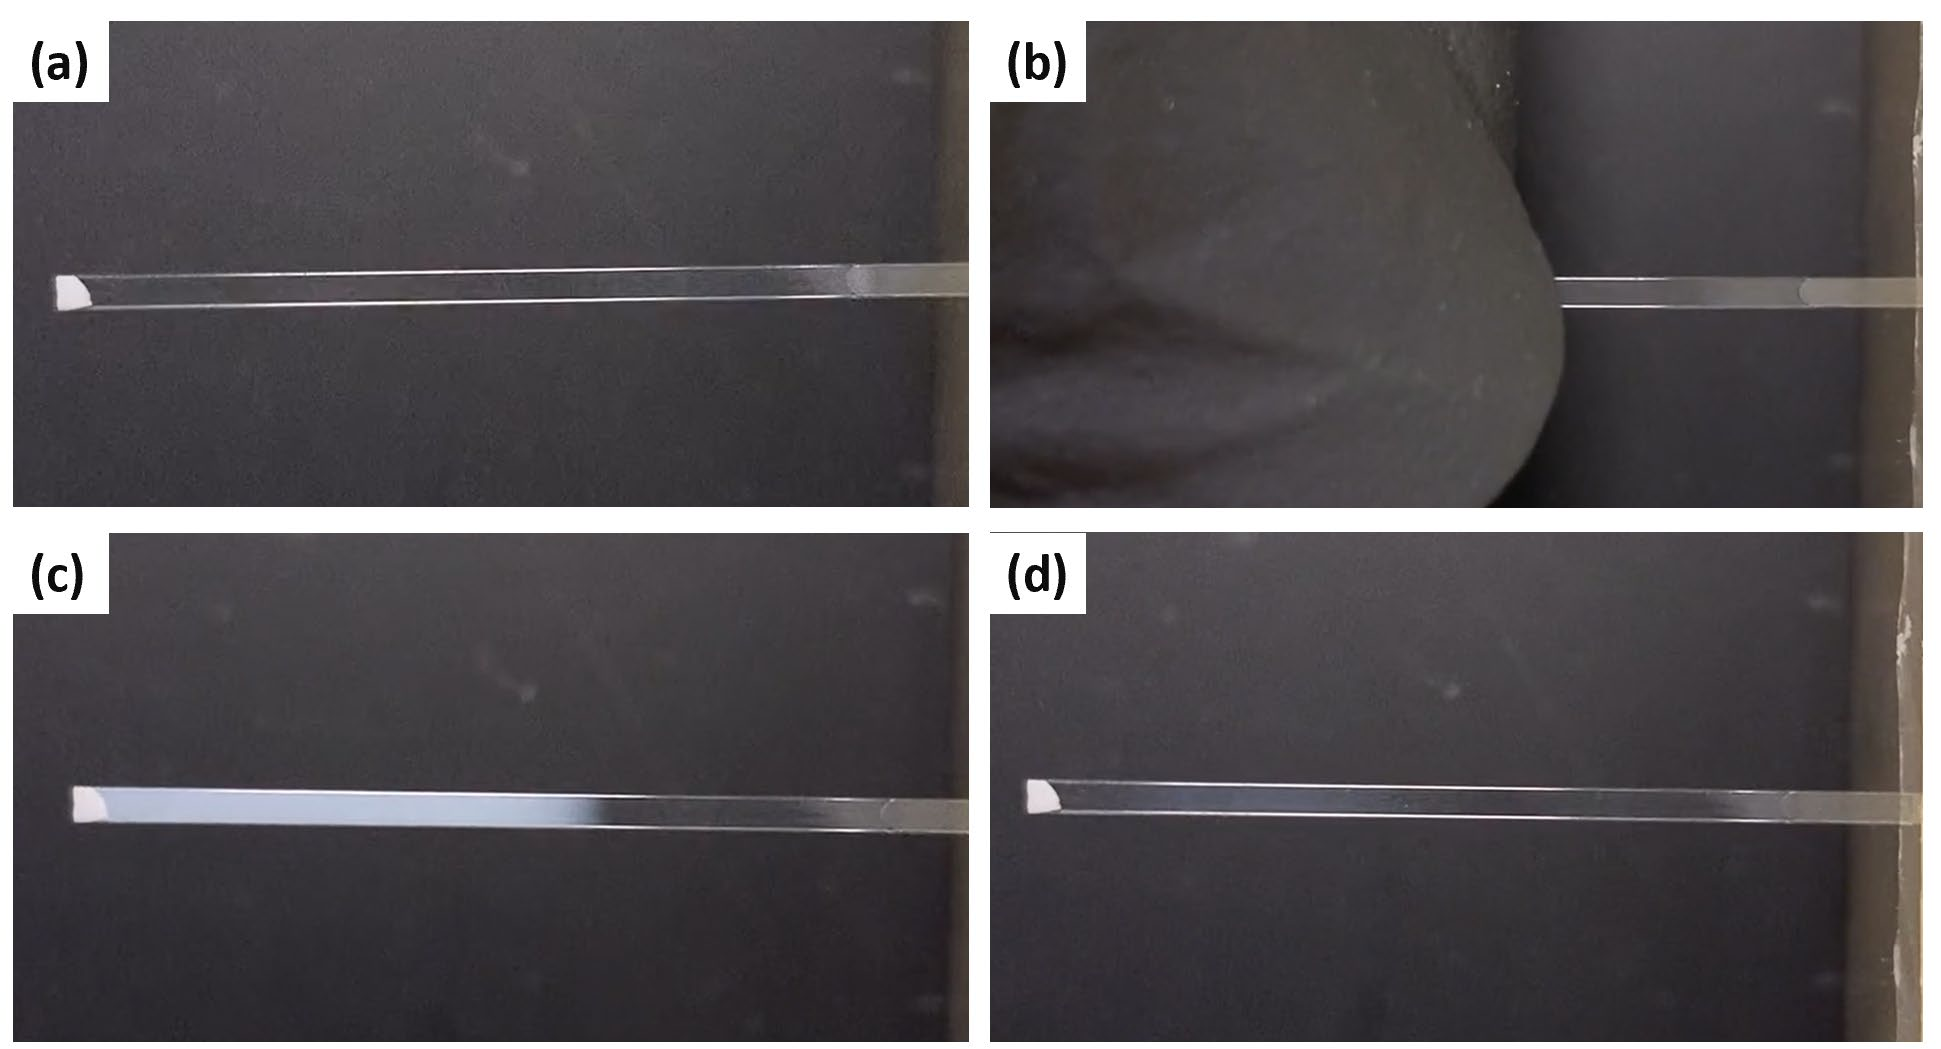
\includegraphics[width=\linewidth]{VideoS1_Stills.jpg}
  \caption{Reversible phase transition in \VP{30}, stills from the video. (a) A thin quartz capillary containing \VP{30} is held in a fixture. (b) The capillary is warmed for about \SI{5}{\second} between thumb and index finger through nitrile gloves. (c) The solution becomes visibly cloudy as sub-micrometer structures form. (d) About \SI{60}{\second} after the heat source is removed, the sample is transparent again. Full video: \url{https://anl.box.com/s/lsukldjnr45nhfrkobijsar1tqhba7jw}.}
  \label{vid:reversible}
\end{video}

\begin{video}[p]
  \centering
  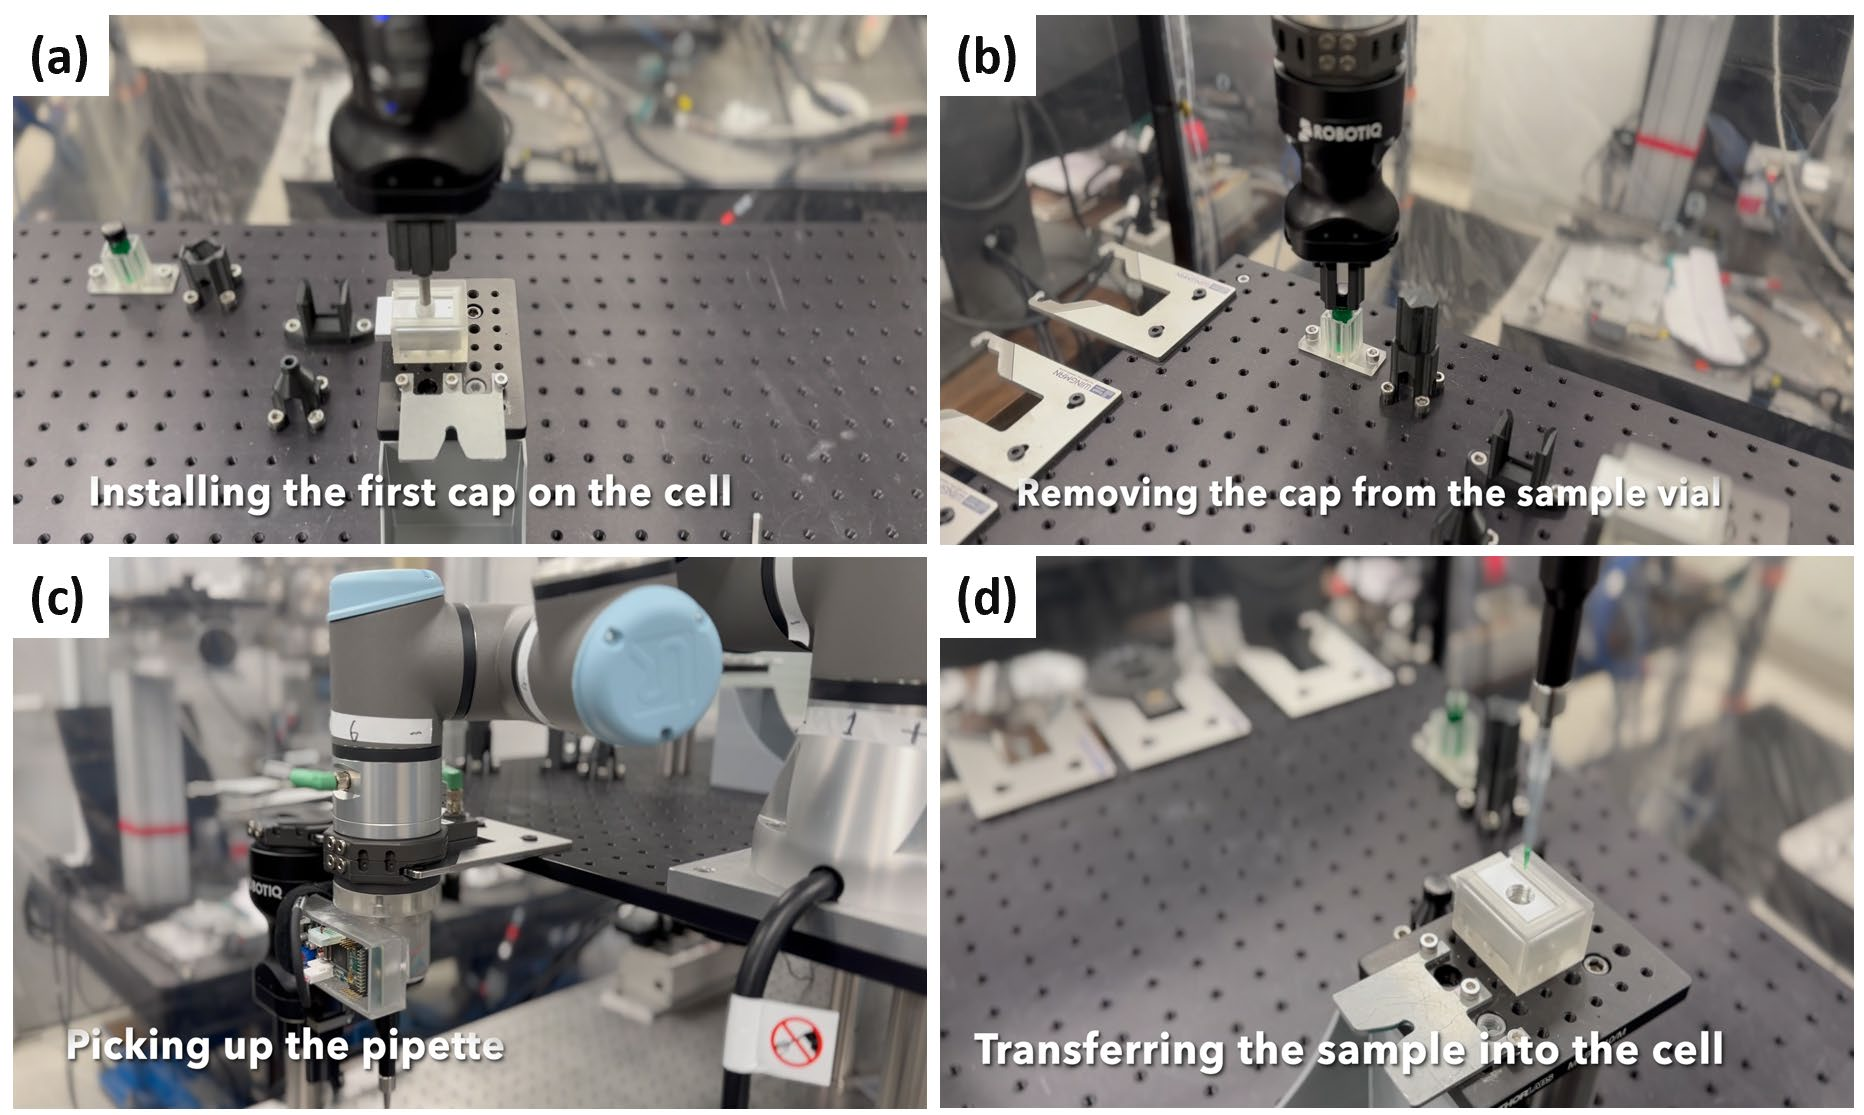
\includegraphics[width=\linewidth]{VideoS2_Stills.jpg}
  \caption{Automated liquid-cell assembly with a six-axis robot and exchangeable end effectors, stills from the video. (a) The UR3e robot with a finger gripper drives the first cap into the cell. The screwdriver handle and the gripper fingers are 3D-printed to match each other's contour, and a locking ring at the tip of the hex bit keeps the polycarbonate cap from falling during transfer. (b) The robot opens a \SI{3}{\milli\liter} glass vial with a twist cap; the grooves of the gripper and of the vial holder are padded with Silastic tubing for friction. (c) The robot exchanges the finger gripper for the electronic pipette through a tool changer that locks mechanically, with no compressed air. (d) The robot transfers the liquid sample into the reservoir formed by the \SI{3}{\milli\meter} through-hole and the first cap; closing the top with the second cap completes the cell. Full video: \url{https://anl.box.com/s/lsukldjnr45nhfrkobijsar1tqhba7jw}.}
  \label{vid:robot}
\end{video}

% the two videos first, as in the Overleaf Supporting Information
\clearpage

\begin{figure}[p]
  \centering
  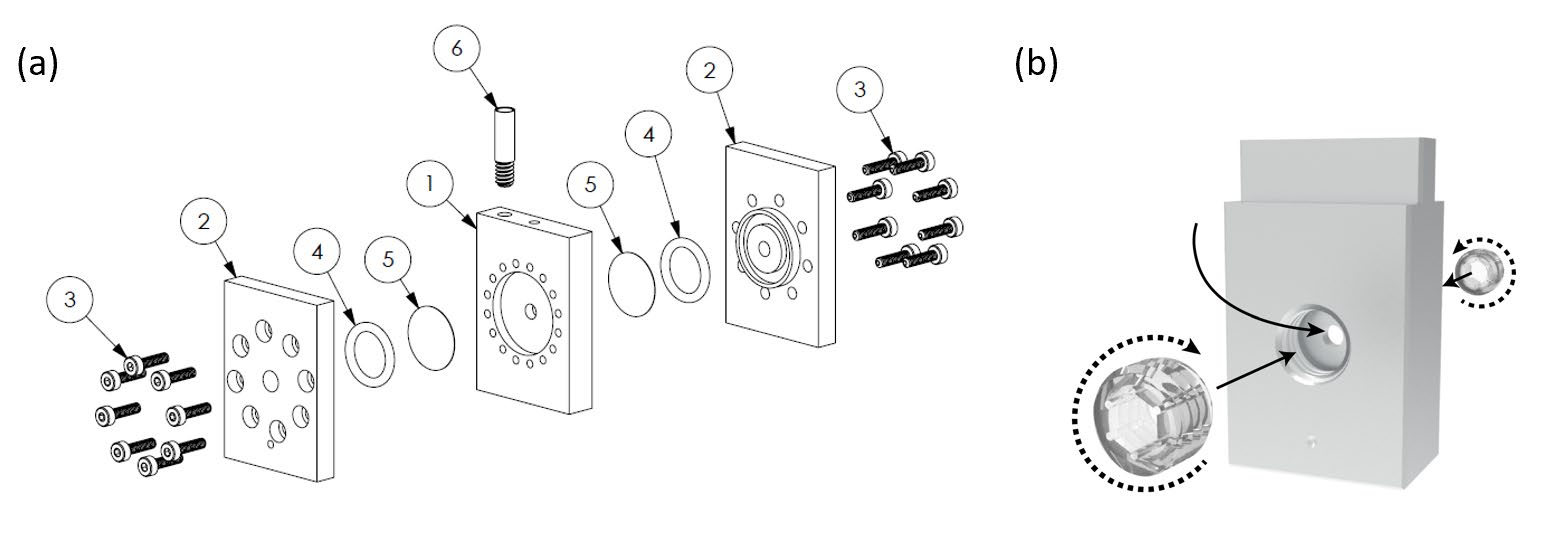
\includegraphics[width=\linewidth]{FigureS1_Sample_Cells.jpg}
  \caption{Assembly of the liquid cells. (a) The cell used for the temperature-induced gelation studies. Assembly requires punching circular windows from Kapton or polycarbonate sheet, inserting O-rings into the grooves of the metallic caps, and bolting the cell on both sides with 16 screws. (b) The cell used for robotic assembly. Its body is machined from a single piece of metal, which removes the variation in exterior contour that uneven O-ring compression produces, and it is closed by torquing CNC-machined, vapor-polished polycarbonate caps into both ends.}
  \label{fig:cells}
\end{figure}

\begin{figure}[p]
  \centering
  \acsfig{FigureS2_Ramp_VPAVG10.pdf}
  \caption{Evolution of structure and dynamics of \VP{10} during heating (left) and the cooling that followed (right). (a, b) Temperature of every acquisition against elapsed time. (c, d) Buffer-subtracted SAXS intensity $I(Q)$ on the absolute scale, one curve per section of 278 acquisitions. (e, f) Intensity autocorrelation function $g_2$ at $Q=\SI{0.0038}{\angstrom^{-1}}$ for the same sections. Color is the mean temperature of the section, on one scale for both columns. The curve of the cooling section at \SI{26.3}{\degreeCelsius} is not drawn in (f) (see text).}
  \label{fig:ramp10}
\end{figure}

\begin{figure}[p]
  \centering
  \acsfig{FigureS3_Ramp_VPAVG20.pdf}
  \caption{Evolution of structure and dynamics of \VP{20} during heating (left) and cooling (right), as in Figure~\ref{fig:ramp10}, with twenty sections of 119 or 120 acquisitions per ramp.}
  \label{fig:ramp20}
\end{figure}

\begin{figure}[p]
  \centering
  \acsfig{FigureS4_Ramp_VPAVG30.pdf}
  \caption{Evolution of structure and dynamics of \VP{30} during heating (left) and cooling (right), as in Figure~\ref{fig:ramp10}, with ten sections of 119 or 120 acquisitions per ramp. The $g_2$ curves of the seven coldest heating sections and the two coldest cooling sections are not drawn: the coherent intensity at this $Q$ is too weak there for a correlation function to be resolved. The heating profiles in (c) are those of Figure~\ref{MT-fig:saxs}a.}
  \label{fig:ramp30}
\end{figure}

\begin{figure}[p]
  \centering
  \acsfig{FigureS5_12ID_Reversibility.pdf}
  \caption{Reversibility of thermally induced gelation in \VP{30}, from SAXS and WAXS at APS 12-ID-B. (a) Merged SAXS and WAXS profiles of two aliquots of the same stock in \SI{2}{\milli\meter} quartz capillaries, at 10 and \SI{30}{\degreeCelsius}. The Measurement aliquot (markers) had been through more than ten heating and cooling cycles; the Reference aliquot (lines) had remained at \SI{4}{\degreeCelsius}. (b) Guinier plot of the Reference aliquot at \SI{10}{\degreeCelsius} with the weighted fit over $0.020\leq Q\leq\SI{0.055}{\angstrom^{-1}}$. The fitted radius of gyration is the characteristic length of the dispersed state used for $\xi(T)$ in Figure~\ref{MT-fig:saxs}b.}
  \label{fig:12id}
\end{figure}

\begin{figure}[p]
  \centering
  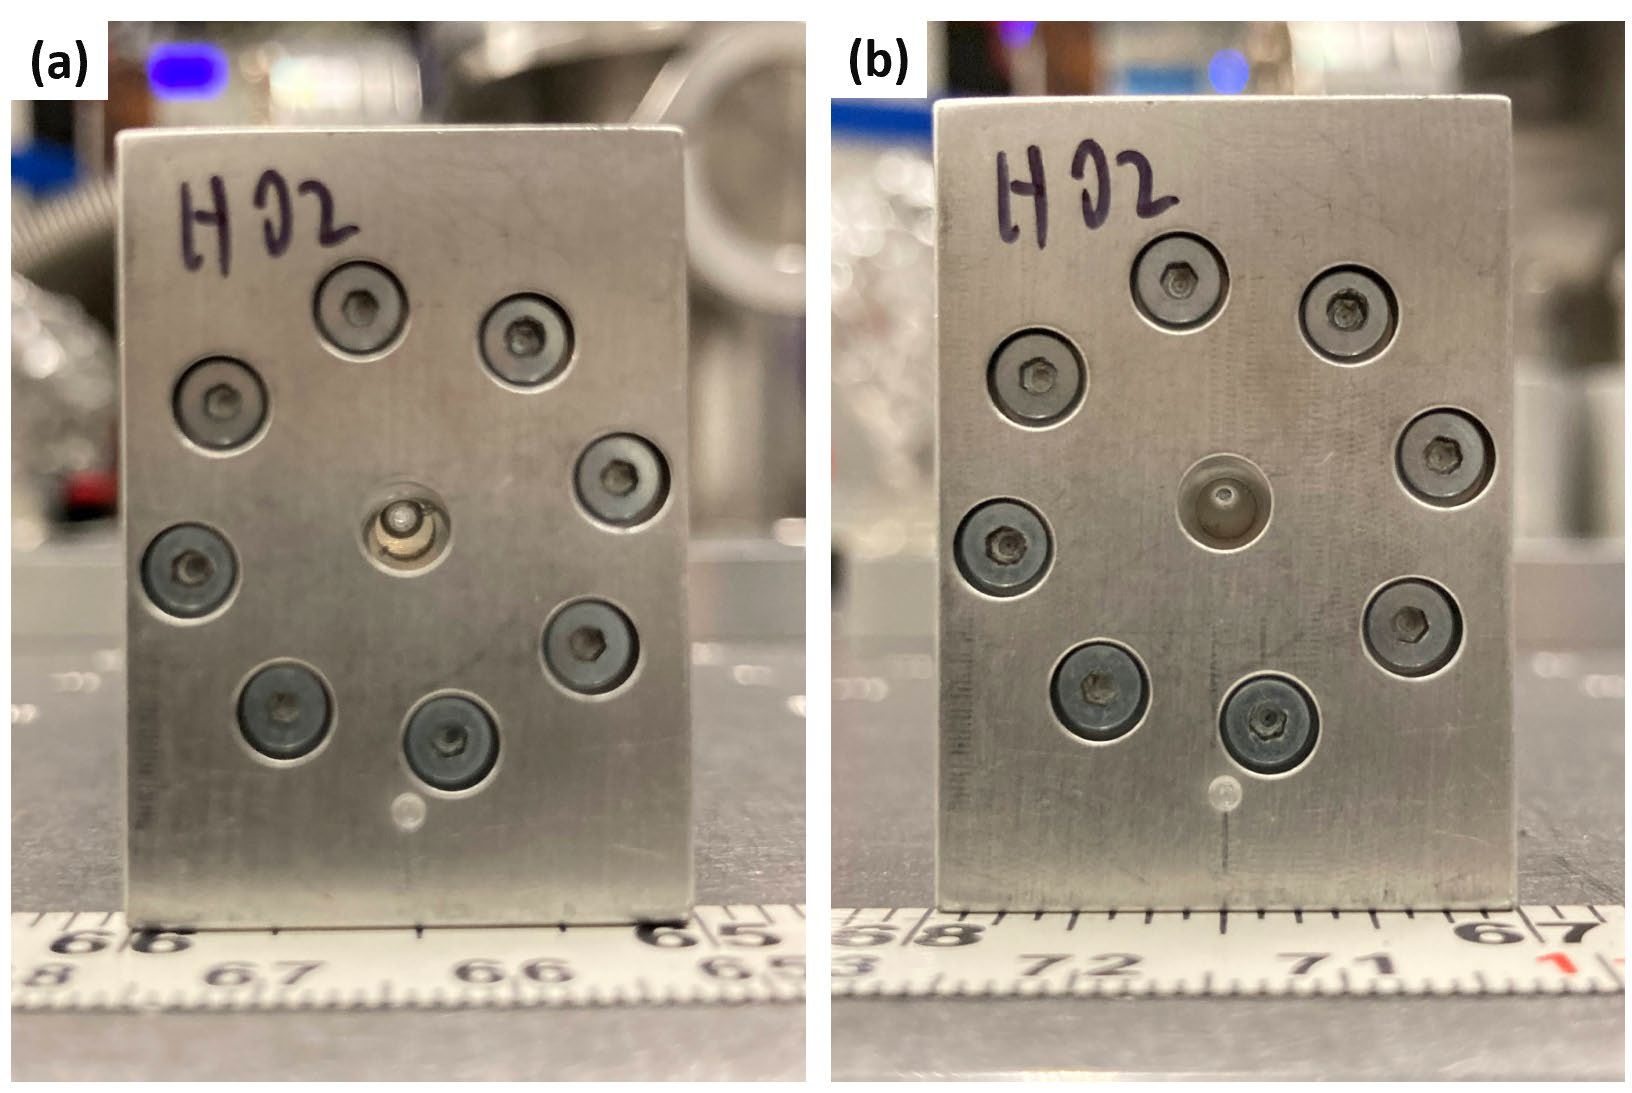
\includegraphics[width=0.85\linewidth]{FigureS6_Irreversibility.jpg}
  \caption{Irreversibility of thermally induced gelation in \VP{10}. (a) The metallic liquid cell containing \VP{10} before the temperature ramp of Figure~\ref{fig:ramp10}. (b) The same cell after the ramp and more than \SI{48}{\hour} in a refrigerator at \SI{4}{\degreeCelsius}. The sample remains opaque.}
  \label{fig:irrev}
\end{figure}

\begin{figure}[p]
  \centering
  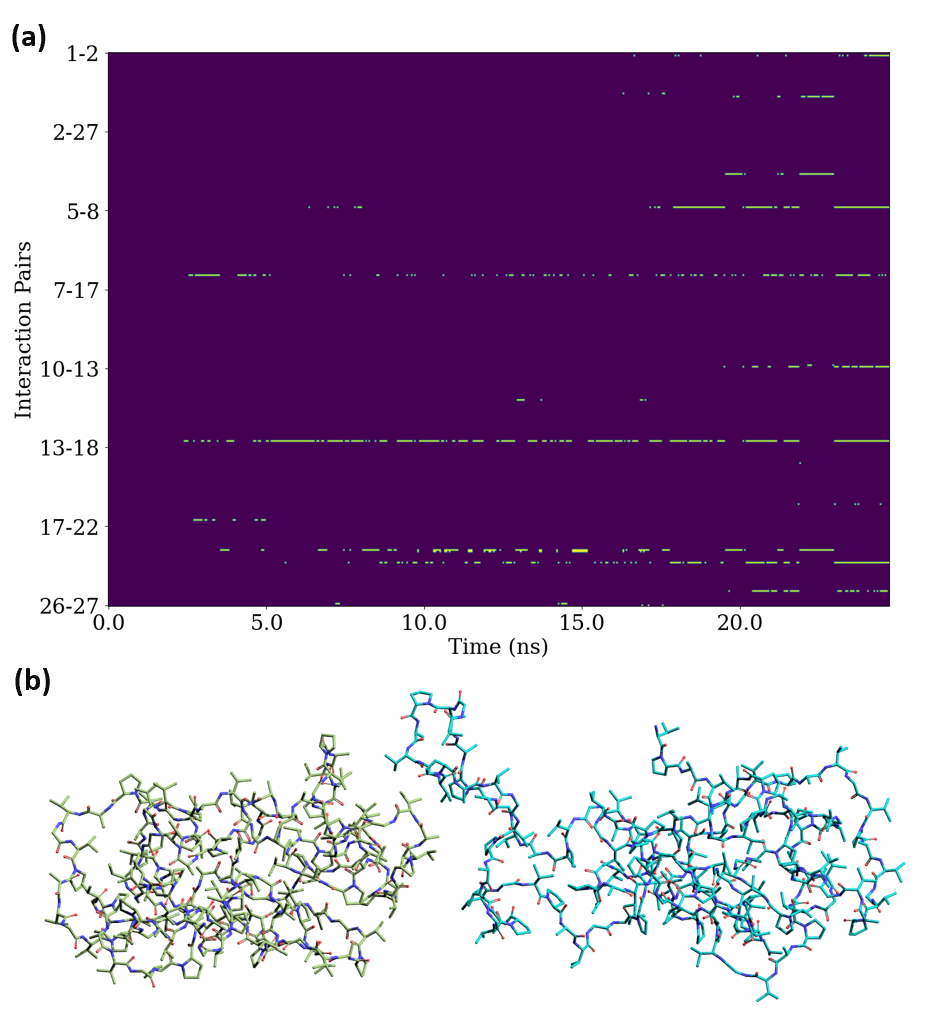
\includegraphics[width=0.75\linewidth]{FigureS7_MD.png}
  \caption{Molecular dynamics simulation of a $3\times3\times3$ cuboidal array of \VP{30}. (a) Contact timeline between pairs of chains: a bright line marks contact, with simulation time along $x$ and the index of the chain pair along $y$. (b) Snapshot of two chains in contact.}
  \label{fig:md}
\end{figure}

\begin{figure}[p]
  \centering
  \begin{minipage}{0.92\linewidth}
  \small
  \textbf{A1 (forward)}\quad \texttt{5$'$-GTTCCAGCTGTTGGTG}\\[4pt]
  \textbf{A2 (reverse)}\quad \texttt{5$'$-ACCTACTGCTGGTACG}\\[4pt]
  \textbf{B1 (forward)}\quad \texttt{5$'$-TACTTCCAATCCAATGCCGTTCCAGCTGTTGGTGTGCCG}\\[4pt]
  \textbf{B2 (reverse)}\quad \texttt{5$'$-TTATCCACTTCCAATGTTAACCTACTGCTGGTACGCCGAC}\\[4pt]
  \textbf{VPAVG OERCA single-stranded template}\\
  \texttt{/5Phos/GTTCCAGCTGTTGGTGTGCCGGCCGTGGGCGTGCCTGC}\\
  \texttt{GGTGGGCGTCCCGGCGGTCGGCGTACCAGCAGTAGGT}
  \end{minipage}
  \caption{Oligonucleotide primers and the 5$'$-phosphorylated single-stranded OERCA template used to construct the ELP genes.}
  \label{fig:sequences}
\end{figure}

\begin{figure}[p]
  \centering
  \acsfig{FigureS9_IC_Calibration.pdf}
  \caption{Conversion of the SAXS intensity to an absolute scattering cross section with the upstream and downstream ion chambers. (a) Photon count measured by a PIN diode against the upstream ion-chamber reading across the attenuation series, with the linear fit used to convert the ion-chamber signal to incident flux. The unattenuated point lies off the line defined by the others and is not shown or fitted. (b) Transmission of the air path between the upstream and downstream ion chambers across the same seven measurements, and its mean.}
  \label{fig:ic}
\end{figure}

\begin{figure}[p]
  \centering
  \acsfig{FigureS10_SAXS_Stability.pdf}
  \caption{SAXS of single acquisitions shows no radiation-induced structural change. $I(Q)$ of the twelve consecutive subsets of 8{,}333 frames of one \SI{100000}{}-frame acquisition of \VP{10}, (a) the first acquisition of the heating ramp, at \SI{20.0}{\degreeCelsius}, and (b) the last, at \SI{45.2}{\degreeCelsius}. Each subset is restored to its own mean intensity and the twelve are placed on the photons-per-pixel-per-frame scale of the whole acquisition.}
  \label{fig:saxsstab}
\end{figure}

\begin{figure}[p]
  \centering
  \acsfig{FigureS11_XPCS_Stability.pdf}
  \caption{XPCS dynamics remain stable throughout an acquisition. $g_2$ at $Q=\SI{0.0038}{\angstrom^{-1}}$ for the ten heating sections of \VP{10} (Figure~\ref{MT-fig:arrest}), correlated from all 100{,}000 frames of each acquisition (circles), from the first 50{,}000 (squares) and from the last 50{,}000 (triangles). The $y$ axis is capped at 0.98, so a few short-delay points of the coldest sections fall below it.}
  \label{fig:xpcsstab}
\end{figure}

\begin{figure}[p]
  \centering
  \acsfig{FigureS12_Flux_Control.pdf}
  \caption{Varying the X-ray flux does not alter the measured structure or dynamics. (a) SAXS intensity and (b) intensity autocorrelation function of a \SI{20}{\milli\gram\per\milli\liter} \VP{30} sample at four incident fluxes, recovered for each measurement from its upstream ion-chamber reading and keyed in the legend.}
  \label{fig:flux}
\end{figure}

\clearpage
\bibliographystyle{achemso}
\bibliography{reference}

\end{document}
